% !TEX root = ../HonoursThesis.tex

\renewcommand{\chapterlabel}{Chapter}
\chapter{Modular echo state networks}
\label{chap:ESNs}



\section{Reservoir computing}

Reservoir computing separates computation into a fixed, randomly initialized dynamical system - the reservoir - and a trained linear readout. An input sequence drives the reservoir's state through time, and at each step the readout maps that state to a corresponding output sequence (commonly the following datapoint within the same sequence). The readout will then yield a prediction when the reservoir is driven with unseen data. Because only the readout weights are learned, training is more efficient than similar models for computing with sequential data, which often require compute-intensive parameter tuning algorithms~\cite{jaeger_2001}. While the reservoir is usually simulated, reservoir computing can act as a model for \textit{in materio} computing~\cite{dale_2016}, in which a reservoir can be created from any material or substrate with sufficiently rich dynamics. An early example of \textit{in materio} computing involved using a bucket of water as a reservoir~\cite{fernando_and_sojakka_2003}.

% Reservoir computing is a framework for processing sequential data characterised by a randomly initialised dynamical system called the reservoir. The reservoir's internal dynamics are not fitted in any way, and instead a much simpler readout function is trained to map the reservoir dynamics to the desired output. An input sequence is used to evolve the state of the reservoir in time and the state of the reservoir at each time step is mapped to a data point along another sequence, commonly the following datapoint within the same sequence. The states are mapped by regressing a readout function to produce the desired ouput sequence, which will yield predictions for an unseen input sequence. Treating the reservoir as a `black box' provides an efficient training method in comparison to other methods for computing with sequential data, many of which require compute-intensive parameter tuning algorithms~\cite{jaeger_2001}. While the reservoir is most often a simulated structure, reservoir computing can act as a model for \textit{in materio} computing~\cite{dale_2016}, in which a reservoir can be created from any material or substrate with sufficiently rich dynamics. An early example of \textit{in materio} computing involved using a bucket of water as a reservoir~\cite{fernando_and_sojakka_2003}.

In the discrete case, the evolution of the reservoir's internal state is governed by a state evolution function $f_{RC}$:
\[
    \mathbf{s}(t+1) = f_{RC}(\mathbf{s}(t), \mathbf{x}(t)).
\]
Here $\mathbf{s}(t)$ represents the internal state of the reservoir at time $t$ and $\mathbf{x}(t)$ is the input signal at time $t$. The output of the reservoir can be computed by a `readout' function of the states of the reservoir $f_{out}$:
\[
    y(t) = f_{out}(\mathbf{s}(t)).
\]

\subsection{Echo state networks}

% - Harnessing Nonlinearity: Predicting Chaotic Systems and Saving Energy in Wireless Communication - Herbert Jaeger* and Harald Haas (2004)

Introduced by Jaeger (2001), echo state networks (ESNs) are a form of reservoir computing which uses a recurrent neural network (RNN) as the reservoir~\cite{jaeger_2001}. RNNs were designed for sequence-to-sequence prediction~\cite{lukosevicius_and_jaeger_2009}, and are often comprised of a single `hidden layer' of states, which undergo the state update equation
% \begin{equation*}
% \mathbf{s}(t+1) = \sigma (\mathbf{C_{in}} \mathbf{x}(t) + \mathbf{C_{rec}} \mathbf{s}(t) + \mathbf{\mathbf{b}})
% \end{equation*}
\begin{equation*}\label{eq:esn_state_update}
    \mathbf{s}(t + 1) = f_{act}\bigl(\mathbf{W}_{in}\mathbf{x}(t) + \mathbf{W}_{rec}\mathbf{s}(t) + \mathbf{W}_{bias}\bigr).
\end{equation*}
The input matrix $\mathbf{W}_{in}$ maps the input signal $\mathbf{x}(t)$ to the network states at each time step $t$, while the recurrence matrix $\mathbf{W}_{rec}$ governs the interactions between states of the network at each time step. The bias vector $\mathbf{W}_{bias}$ is added at each time step, and the resulting values are passed through a nonlinear activation function, $f_{act}$, where it is common to use the $tanh$ function.

One can generate a prediction $\mathbf{\hat{y}}(t)$ at time $t$ by multiplying the scalar product of the state vector $\mathbf{s}(t)$ and the readout vector $\mathbf{C}_{out}$,
\[
    \mathbf{\hat{y}}(t) = \mathbf{C}_{out}\mathbf{s}(t).
\]
After we have used the input time series $\mathbf{x}(t)$ to create the state $\mathbf{s}(t)$ at each time step $t$, it is convenient to generate predictions over the whole time series at once. By combining the states into a matrix $\mathbf{S}$ we can derive all predictions $\mathbf{\hat{y}}(t)$ combined into a single vector~$\mathbf{\hat{Y}}$:
\[
    \mathbf{\hat{Y}} = \mathbf{C}_{out}\mathbf{S}.
\]
A diagram of an ESN can be found in Figure \ref{fig:ESN}.

\begin{figure}
    
    \centering
    \begin{tikzpicture}[scale=1.2]
        \node[fill=black,circle,inner sep=2pt,label=left:$\mathbf{x}(t)$] (input) at (0,0) {};
        \node[fill=black,circle,inner sep=2pt,label=right:$\mathbf{\hat{y}}(t)$] (output) at (10,0) {};
        
        
        \coordinate (res_anchor) at (2,3);
        \node[fill=black,circle,inner sep=2pt] (res1) at ({5-0.5},{0.8}) {};
        \node[fill=black,circle,inner sep=2pt] (res2) at ({5},{-1}) {};
        \node[fill=black,circle,inner sep=2pt] (res3) at ({5},{0.15}) {};
        \node[fill=black,circle,inner sep=2pt] (res4) at ({5+1},{-0.1}) {};
        \node[fill=black,circle,inner sep=2pt] (res5) at ({5-0.75},{-0.5}) {};
        \node[fill=black,circle,inner sep=2pt] (res6) at ({5-1.25},{0.4}) {};
        \node[fill=black,circle,inner sep=2pt] (res7) at ({5+0.65},{0.75}) {};
        \node[fill=black,circle,inner sep=2pt] (res8) at ({5+1},{-0.9}) {};
        \node[fill=black,circle,inner sep=2pt] (res9) at ({5-1.25},{-1}) {};
        \node[fill=black,circle,inner sep=2pt] (res10) at ({5-1.75},{-0.25}) {};
    
        \foreach \i in {1,...,10}
            \draw[gray,line width=0.1] (input) -- (res\i);
        
        \foreach \i in {1,...,5}
            \foreach \j in {1,...,5} {
                \ifnum\i<\j
                    \draw (res\i) -- (res\j);
                \fi
            }
        
        \draw (res6) -- (res5);
        \draw (res6) -- (res1);
        \draw (res6) -- (res10);
        \draw (res10) -- (res5);
        \draw (res9) -- (res10);
        \draw (res9) -- (res2);
        \draw (res7) -- (res1);
        \draw (res7) -- (res3);
        \draw (res7) -- (res4);
        \draw (res8) -- (res4);
        \draw (res8) -- (res2);
        
        \foreach \i in {1,...,10}
            \draw[gray,line width=0.1] (res\i) -- (output);
        
        \begin{scope}[on background layer]
        \draw[draw=black,fill=pale_yellow,rounded corners=8pt]  ($(res1)+(-0.1,0.3)$) -- ($(res7)+(+0.2,+0.2)$) -- ($(res4)+(0.4,0)$) -- ($(res8)+(0.2,-0.2)$) -- ($(res2)+(0,-0.2)$) -- ($(res9)+(-0.2,-0.2)$) -- ($(res10)+(-0.3,0)$) -- ($(res6)+(-0.3,0)$) -- cycle;
        \end{scope}
        \node at (5.2, 1.4) {$\mathbf{W}_{\text{rec}}$};
        \node at (5, -1.6) {$\mathbf{s}(t)$};
        
        \draw[fill=white,opacity=0.8] (1.2,-0.75) rectangle (2.0,0.75) node[midway] {$\mathbf{W}_{\text{in}}$};
        \draw[fill=white,opacity=0.8] (8, -0.75) rectangle (8.8,0.75) node[midway] {$\mathbf{C}_{\text{out}}$};
    \end{tikzpicture}
    \caption{A diagram of an echo state network. The points labeled $\mathbf{x}(t)$ and $\mathbf{\hat{y}}(t)$ are the input and prediction respectively. The other points represent the states $\mathbf{s}(t)$ of the network. The lines represent the multiplications of the weighting vectors with $\mathbf{x}(t)$ and $\mathbf{s}(t)$ in equation \ref{eq:esn_state_update}.}
    \label{fig:ESN}
\end{figure}

In conventional RNNs, the parameters $\mathbf{W}_{in}$, $\mathbf{W}_{rec}$, and $\mathbf{C}_{out}$ are typically optimised during training; however, for echo state networks, this is not the case.
ESNs will randomly instantiate $\mathbf{W}_{in}$ and $\mathbf{W}_{rec}$ and keep them fixed, while simply fitting the readout vector $\mathbf{C}_{out}$. One could do so using ordinary least squares regression, where the coefficients of $\mathbf{C}_{out}$ are chosen to minimise the sum of squared errors
\[
\min_{\mathbf{C}_{out}} \;\bigl\lVert \mathbf{S}\,\mathbf{C}_{out} - \mathbf{Y}\bigr\rVert_2^2,
\]
however it is beneficial to use ridge regression instead~\cite{lukosevicius_2012_practical_guide}, augmenting the objective with an \(\ell_2\) penalty on the coefficients yielding the loss function
\[
\min_{\mathbf{C}_{out}}\;\bigl\lVert \mathbf{S}\,\mathbf{C}_{out} - \mathbf{Y}\bigr\rVert_2^2
\;+\;\beta\,\bigl\lVert \mathbf{C}_{out}\bigr\rVert_2^2.
\]
This regularises the readout vector, making the predictions stable for unseen reservoir states and preventing numerical instability. The regularisation parameter $\beta$ controls the penalty imposed on large-magnitude coefficients in the output matrix $\mathbf{C}_{out}$~\cite{lukosevicius_2012_practical_guide}. Because the loss function is strictly convex, there is a closed-form solution:
\[
    \mathbf{C}_{out}^T = (\mathbf{S}^T \mathbf{S} + \beta \mathbf{I}) \ \mathbf{S}^T \mathbf{Y}.
\]
It is generally fast to find the solution to this linear equation and it yields a readout that generalises stably to unseen reservoir states.

The bias vector $\mathbf{W}_{bias}$ and input weight matrix $\mathbf{W}_{in}$ are simply instantiated with values drawn from a random distribution such as a Normal distribution. The recurrence matrix $\mathbf{W}_{rec}$ is generated using a random graph generation algorithm such as an Erd\H{o}s-R\'enyi sparsely connected random graph with nodes $k$ and average degree $d$, producing a $k \times k$ matrix. To rescale the magnitudes of the recurrence matrix based on the `spectral radius' parameter $\rho$, one would find the maximum absolute eigenvalue of the matrix $\lambda_{max}$, and scale the matrix like so:
\[
\mathbf{W}_{rec} \leftarrow \mathbf{W}_{rec}\frac{\rho}{\lambda_{max}}.
\]
The states $\mathbf{s}(0)$ are initialised as a vector of values drawn from a random distribution such as the normal distribution $\mathcal{N}(0, 1)$.

\subsection{Computational efficiency}

Increasing the number of states ($k$) in a traditional RNN significantly escalates the computational load during training due to the quadratic increase in the number of parameters that must be optimised. In contrast, ESNs avoid this issue as the vast majority of their parameters remain fixed. Thus, ESNs have a computational efficiency during parameter optimisation, although this advantage does not extend to the inference phase, when predictions are generated.

Fitting the parameters of an RNN requires accounting for errors propagating through time, often using the Backpropagation Through Time algorithm~\cite{lukosevicius_and_jaeger_2009}. However, this training method is costly and the successive multiplication of extreme numbers (large and small) causes the gradients calculated through this algorithm to either `vanish' or `explode'~\cite{lukosevicius_and_jaeger_2009}. While some RNNs such as Long Short-Term Memory (LSTM) networks encode a memory buffer to mitigate this problem~\cite{hochreiter_1997}, reservoir computers offer another alternative. Since ESNs avoid fitting the recurrence matrix and the input vector, they can take advantage of a large number and depth of parameters without suffering from the issues of vanishing gradients. While ESNs have the added benefit of requiring far less training computation than traditional RNNs, they require some care to be taken in establishing the properties of the reservoir.

\subsection{The echo state property}

The defining characteristic of reservoir computers is the \textit{echo state property}. This property ensures that, given a sufficiently long input sequence, the current state of the reservoir is determined uniquely by the intervening input and is independent of its initial state~\cite{jaeger_2001}. In other words, the further past inputs are in time from the current state, the less they impact the current state. More formally, a network possesses echo states if its states are uniquely determined by the input sequence $\mathbf{x}(t)$ for some sufficiently large $t$, i.e., $\mathbf{s}(t) = \mathbf{s}'(t)$ for any initial states $\mathbf{s}(0)$ and $\mathbf{s}'(0)$, where $\mathbf{s}(t)$ represents the reservoir state at time $t$ and the states are evolved with the same weights $\mathbf{W}_{in}$ and $\mathbf{W}_{rec}$.

For a network to exhibit the echo state property, it must satisfy three key conditions~\cite{buehner_young_2006}:
\begin{itemize}
    \item \textbf{Uniform State Contraction:} The network must be contractive, meaning that differences in initial states decay over time.
    \item \textbf{State Forgetting:} The network must `forget' its initial state after a finite amount of time, ensuring that only recent inputs affect the current state.
    \item \textbf{Fading Memory:} The influence of past inputs diminishes over time, making the network's state primarily a function of recent inputs.
\end{itemize}

With each condition satisfied, the ESN will exhibit the echo state property and thus holds a limited \textit{memory capacity}. Each state of the network can be viewed as a function of a finite sequence of prior inputs:

\begin{align*}
\mathbf{s}(t) &= \mathcal{F}(\mathbf{s}(t-1), \mathbf{s}(t-2), ... \mathbf{s}(0)) \\
&\approx \mathcal{F}(\mathbf{s}(t-1), \mathbf{s}(t-2), ... \mathbf{s}(t-\tau_{MC})),
\end{align*}
where the number of time steps $\tau_{MC}$ corresponds to some memory capacity of the network. The states that are beyond $\tau_{MC}$ steps in the past practically do not contribute to $\mathbf{s}(t)$. The memory capacity for a given time delay $\tau_{max}$ can be quantified by the following method as proposed by Jaeger (2001)~\cite{jaeger_2001}:
\begin{equation*}
    MC(\tau_{max}) = \sum^{\tau_{max}}_{\tau=1} Corr\bigg[\big\{\mathbf{x}(n-\tau), \mathbf{\hat{y}}_\tau(n)\big\}_{n=\tau}^{n=T}\bigg]^2.
\end{equation*}
The input sequence $\mathbf{x}$ is I.I.D. noise, and the series $\mathbf{\hat{y}}_\tau$ refers to the outputs of a reservoir computer trained to reproduce the input sequence after $\tau$ time steps have elapsed. We are calculating the Pearson correlation of these `remembered' values with the input values over the whole sequence, where $T$ is the final time step of the sequence. To measure the length of the reservoir computer's memory $\tau_{MC}$, we should find the lowest value of $\tau_{max}$ for which the memory capacity has approximately converged. This value will represent how many time steps in the past a reservoir computer can recall patternless inputs. In later publications, the calculation of memory capacity is performed by summing the correlations directly, without squaring them first~\cite{lukosevicius_and_jaeger_2009}.

In most prediction tasks, the most recent inputs are more relevant than those received further into the past. This is the intuitive justification for why the echo state property is important to creating a useful model. With a large enough memory capacity, the echo state property ensures that the reservoir provides a rich, yet stable and decaying, representation of the input signal over time.

By scaling the recurrence matrix $\mathbf{W}_{rec}$ so that its spectral radius equals our parameter $\rho$, we are controlling the effect of the states $s(t)$ on the states $s(t+1)$ relative to the input signal $x(t+1)$. By scaling $\mathbf{W}_{rec}$ by $\rho$, we are regulating the reservoir's decay rate of past activations and thus its memory capacity. When $0 < \rho < 1$, the past states are propagated through the network but the current input is still the dominant effect on the activation states. As $\rho$ increases, the reservoir begins to exhibit chaotic behavior. As we increase $\rho > 1$, the ESN approaches a tipping point (often referred to as the `edge of chaos') beyond which the ESN memory dominates the input signal. With values $\rho >> 1$, the ESN becomes unstable and uninformative as the input signal has little effect on its dynamics. A commonly used heuristic is to set $\rho \approx 1$ to balance the memory and the stability of the ESN and testing small adjustments (e.g. up and down by 0.05) on validation data~\cite{lukosevicius_and_jaeger_2009}~\cite{lukosevicius_2012_practical_guide}. Generally, tasks requiring a longer memory will require a larger $\rho$.



\section{Mixture-of-experts}

The concept of the `Adaptive Mixture of Local Experts' was originally introduced by Jacobs et al. in 1991~\cite{jacobs_1991}. This approach involves training several neural network modules, referred to as `expert' modules, alongside a `gating network' that uses a softmax function to weight the outputs of these experts. The final output of the system is a weighted combination of the outputs from the expert modules. A general diagram of this model is shown in Figure \ref{fig:MOE}. Both the experts and the gating function are trained concurrently on a supervised task, allowing the system to automatically partition the problem among the experts. This method was shown to achieve better generalization compared to a monolithic network~\cite{jacobs_1991}.

Mixture of experts (MOEs) can be viewed as a specialised form of ensemble learning~\cite{masoudnia_2014}. Ensemble learning methods such as bagging, boosting and stacking also combine the outputs of multiple models to improve the prediction of any single model. However the MOE does so with an adaptive and input dependent weighting supplied by the gating function rather than fixed or globally learned weights. This conditional routing lets the MOE weight experts more in the areas of the data where they are most competent. Bias-variance-covariance analysis shows that the selection of local experts trims bias and covariance, whereas the averaging of experts suppresses variance, and the best generalisation arises when the gate balances the two strategies~\cite{masoudnia_2014}. Jointly training the gating function and the experts encourages negatively correlated errors among the experts, whose mutual cancellation reduces ensemble error more effectively than uncorrelated (but unbiased) predictors~\cite{masoudnia_2014}.

% Furthermore, MOE models can be viewed as a generalisation of piecewise models and gating methods known beforehand. Models in which the gating function is rule-based are special cases of MoE where the gating function is defined by some known criterion, rather than being trained or fitted alongside the experts.

Furthermore, MOEs may be seen on a spectrum that spans deterministic piece-wise models, rule-based gating schemes, and fully adaptive probabilistic gates. At one extreme, the gate is specified explicitly by decision rules and each expert is tied to a fixed partition of the input space so that the model behaves as a piece-wise approximator~\cite{masoudnia_2014}. At the other extreme, the gate and the experts are trained jointly, where the gate supplies smooth, input-dependent weights that encourage negatively correlated errors and an arbitrarily complex partitioning of input space.

While fully adaptive gates trained alongside the experts provide a flexible and generally effective method of partitioning the input space, rule based gating allows the modeller to encode a priori knowledge of the time series directly into the gate. This prior decomposition avoids the common difficulty of fitting the gating function on complex and nested boundaries between experts by tying one expert to each predefined region~\cite{masoudnia_2014}. Because the gate's decision logic is deterministic and transparent, the mapping from the input region to the expert remains human readable. A practical bonus is computational: once the split is set, every expert can be trained independently and in parallel. For ESNs this means the model as a whole still enjoys the original efficient training afforded by a handful of ridge regressions.

\usetikzlibrary{arrows.meta, positioning}
\begin{figure}[h]
    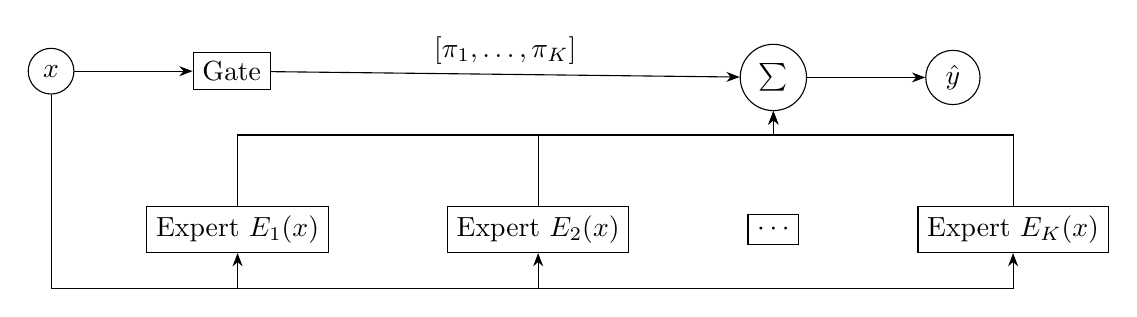
\begin{tikzpicture}[node distance=1.5cm and 1.5cm, >=Stealth]

        % Nodes
        \node (input) [draw, circle] {\(x\)};
        \node (gate) [draw, rectangle, right=of input] {Gate};
        \node (expert1) [draw, rectangle, below right=1.5cm and 1cm of input] {Expert \(E_1(x)\)};
        \node (expert2) [draw, rectangle, right=of expert1] {Expert \(E_2(x)\)};
        \node (expert3) [draw, rectangle, right=of expert2] {\(\cdots\)};
        \node (expertK) [draw, rectangle, right=of expert3] {Expert \(E_K(x)\)};
        \node (sum) [draw, circle, above=1.3cm of expert3] {\(\sum\)};
        \node (output) [draw, circle, right=of sum] {\(\hat{y}\)};
        
        % Connections
        \draw[->] (input) -- (gate);
        \draw[->] (input) |- ([yshift=-0.75cm]expert1.center) -- (expert1.south);
        \draw[->] (input) |- ([yshift=-0.75cm]expert2.center) -- (expert2.south);
        \draw[->] (input) |- ([yshift=-0.75cm]expertK.center) -- (expertK.south);

        % \draw[->] (gate) -- (sum);
        \draw[->] (gate) -- node[above] {$[\pi_1, \dots, \pi_K]$} (sum);
        
        \draw[->] (expert1) -- ++(0,1.2) -| (sum);
        \draw[->] (expert2) -- ++(0,1.2) -| (sum);
        \draw[->] (expertK) -- ++(0,1.2) -| (sum);
      
        \draw[->] (sum) -- (output);
        
      \end{tikzpicture}
      \caption{A general diagram of a MOE model. Each expert $E_i(x)$ is weighted by $\pi_i$ for a given input $x$ for $i \in 1...K$.}
      \label{fig:MOE}
\end{figure}

The structure of this approach can be visualised as a tree, comprising three main components:

\begin{itemize}
    \item multiple expert models, which can be either regression functions or classifiers;
    \item a gate that creates partitions of the input space, defining regions for each individual expert; and
    \item a probabilistic model that combines the outputs of the experts and the gate.
\end{itemize}

This model introduces three important properties: it allows individual experts to specialize in smaller parts of the larger problem, uses soft partitions of the data, and enables splits of the input space along hyperplanes at arbitrary orientations~\cite{jordan_1994}. This approach is particularly beneficial for handling nonstationary data, where the time series switch their dynamics in different regions of the input space~\cite{yuksel_2012}.

Jordan (1994) formalised the `Hierarchical Mixture of Experts' (HME) model, and provided an Expectation-Maximisation (EM) algorithm for its training~\cite{jordan_1994}. The EM algorithm is an iterative two-step procedure for fitting models with latent variables, and alternates between the Expectation (E) step and Maximisation (M) step. For MOE models, the E step computes a set of normalised posterior weights for each data point that reflect how well each expert (given the current gate and expert models) explains that data point. Then the M step updates the gate to predict those posterior weights and retrains each expert, weighting the importance of each data point to each expert by the posterior weights. Iterating these steps leads to convergence: the gating network assigns higher weights to the most accurate experts for each input and each expert's parameters are optimised with respect to the data weighted by those assignments. The HME model allows gating to be organised in a tree like hierarchy of multiple levels of experts, enabling a more complex partitioning of the input space and can lead to improved performance on tasks where the data exhibits hierarchical or multi-scale characteristics~\cite{jordan_1994}.

MOE models have been applied to various types of data, including the task of predicting time series. Tabuse, Kinouchi \& Hagiwara (1997) proposed a novel approach that uses a mixture of RNNs specifically for time series processing~\cite{tabuse_kinouchi_and_hagiwara_1997}. This method uses the Expectation-Maximisation (EM) algorithm for training, and has been shown to result in faster training times and improved performance on benchmark sequences when compared to a single RNN. A resurgence of interest in the mixture of RNN Experts was marked by a notable paper by Shazeer et al. (2017) titled ``Outrageously Large Neural Networks"~\cite{shazeer_2017}, which demonstrated the effectiveness of using a mixture of experts within a stacked Long Short-Term Memory (LSTM) network - a type of RNN - for machine translation tasks.

In the context of ESNs, Babinec and Posp\'ichal (2009) investigated the concept of a modular ESN. This approach involves using several unconnected ESN reservoirs in parallel as expert models, each possessing different internal dynamics and memory capacities~\cite{babinec_pospichal_2009}. The different dynamics were created by varying the spectral radii and internal connection patterns of the networks. A separate gating network - another ESN - was trained to determine the appropriate weighting of the different reservoir outputs. The modular ESN was tested on a chaotic laser intensity time series, where the dynamics exhibited both fast and slow oscillatory components. The results indicated that the ESN MOE outperformed a single ESN, demonstrating that the gating network could dynamically assign higher weight to the expert whose ``memory length" best matched the current behaviour of the series, thus dynamically adapting the model's time scale. 

 

\section{Modular echo state networks}

Since they were introduced by Jaeger (2001), a taxonomy of different ESNs has grown, from SHESN~\cite{deng_and_zhang_2007}, HESN~\cite{jarvis_2010}, and ConvESN~\cite{ma_2021} to Deep-ESN~\cite{gallicchio_and_micheli_2017}, Mod-DeepESN~\cite{carmichael_2018}, GD-ESN~\cite{li_2022}, gdESN~\cite{wcislo_2021}, MH-ESN~\cite{lun_2023}, IR-ESN~\cite{argentieri_2022} and MSSESN~\cite{ma_chen_2013}.
% Since they were introduced by Jaeger (2001), a taxonomy of different ESNs has grown, from MLESN, MSSESN, IR-ESN, and ConvESN, to DFDs or DRNs.
Many of these proposals use multiple reservoirs - or `sub-reservoirs' - in their design, whether they are arranged hierarchically, in parallel or in some other configuration.

Jaeger (2007) himself proposed the concept of a `Dynamic Feature Discoverer (DFD)', in which multiple ESNs are components of a larger system~\cite{jaeger_2007}. Jaeger arranged multiple ESN modules in a hierarchy, each receiving input from lower level ESNs, with the lowest level ESN receiving the standard input $\mathbf{x}(t)$. This allowed the DFD to capture latent features on different temporal or spatial scales, where the higher level ESNs represent a longer time scale than the lower level ESNs. Each ESN layer produces high dimensional features at each time step, and then finds the scalar multiple between its predicted features and the prediction of the layer above. The outputs are combined and passed down in this way until the final layer produces the overall prediction for that time step.

% A similar model was used by Triefenbach et al. (2010, 2013) for accoustic modelling, where they also trialled a dual reservoir ESN where one sub-reservoir received the signal in chronological order, and one received it in reverse (2013).  double check and rewrite this -- DISCARDED

% DISCARDED
% - Yanbo Xue, Le Yang, Simon Haykin, Decoupled echo state networks with lateral inhibition, Neural Networks 20 (3) (2007) 365-376
%     - 'Decouples' sections of the inner state by:
%         - disconnecting sub-reservoirs, and
%         - using a lateral inhibition unit to create diversity of responses between the sub-reservoirs

Modular echo state networks have since been included in larger ensembles of models, for example Ma et al. (2021) proposed a multi-reservoir solution where the reservoirs run in parallel at different time scales~\cite{ma_2021}. They proposed using convolutional neural networks to analyse the states of the reservoirs and extract relevant features across time. They demonstrated that the ConvESN could successfully perform a variety of classification tasks for sequence based data.


\subsection{Restricted echo state networks}

While there are many `modular' ESNs, Wringe et al. (2024) describes a further niche of `restricted' ESNs~\cite{wringe_2024}. Restricted ESNs have idiosyncrasies within their internal structure, and are not simply assemblies of traditional ESNs. Restricted ESNs divide their internal reservoir states into several smaller sub-reservoir states simply by restricting certain connections within the recurrence matrix $\mathbf{W}_{rec}$. There may also be other deviations from the traditional ESN, but the restriction of the recurrence weights is what makes them modular. The state vector can be seen as the concatenation of sub-reservoir state vectors,
\[
    \mathbf{s} = (\mathbf{s}_1, \mathbf{s}_2...\mathbf{s}_n)
\]
where $\mathbf{s}_i$ represents the states within the sub-reservoir $i$. Thus the recurrence matrix $\mathbf{W}_{rec}$ can be defined in terms of the recurrence matrices of the sub-reservoirs $\mathbf{W}_{i}$ and the connections between these submatrices $\mathbf{W}_{i,j}$:

\[
    \mathbf{W}_{rec} = \begin{pmatrix}
        \mathbf{W}_{1} & \mathbf{W}_{1,2} & \cdots & \mathbf{W}_{1,n} \\
        \mathbf{W}_{2,1} & \mathbf{W}_{2} & \cdots & \mathbf{W}_{2,n} \\
        \vdots & \vdots & \ddots & \vdots \\
        \mathbf{W}_{n,1} & \mathbf{W}_{n,2} & \cdots & \mathbf{W}_{n}
    \end{pmatrix}.
\]

% By defining the structure of the sub-reservoirs through restrictions on the reservoir weight matrix, the input vector $\mathbf{W}_{in}$ and the readout vector $\mathbf{C}_{rec}$ can be defined in the traditional way and other structural idiosyncrocies can be simplified.

An early example of a restricted ESN is the Scale-Free Highly Clustered ESN (SHESN)~\cite{deng_and_zhang_2007}, where each sub-reservoir consists of a number of local neurons clustered around a backbone neuron. These backbone neurons connect the sub-reservoirs to one another. The SHESN outperformed the traditional ESN at approximating complex nonlinear dynamics (the Mackey-Glass system) and displayed an enhanced echo state property~\cite{deng_and_zhang_2007}. Another architecture, the Hierarchically Clustered ESN (HESN), built upon the SHESN by making the sub-reservoirs randomly connected rather than fully connected and allowing for multiple backbone neurons per sub-reservoir~\cite{jarvis_2010}.

Malik et al. (2017) proposed the  MultiLayered Echo State Machine (ML-ESM), where the reservoir is arranged into sequential sub-reservoirs~\cite{malik_2017}. Each sub-reservoir is fully connected to neighbouring sub-reservoirs using fixed weights within the reservoir's recurrence matrix - visualised in Figure \ref{fig:ML_ESM_recurrence_matrix} They demonstrated that the ML-ESM outperforms traditional ESNs in tasks requiring the modelling of complex temporal dependencies.

% \begin{figure}
%     \centering
%     \begin{tikzpicture}[scale=2]
%         \def\n{3}
%         \draw[black] (1,1) rectangle (\n+1, \n+1);
        
%         % \foreach \x in {1,...,\n} {
%         %     \fill[col\x] (\x,\n-\x+1) rectangle ++(1, 1);
%         % }
%         % \def\k{10}
%         % \foreach \x in {1,...,\k} {
%         %     \fill[black!10] (1 + 1+\x/\k-1/\k, 0 + 1+\n-\x/\k) rectangle ++(1/\k, 1/\k);
%         % }
%         % \foreach \x in {1,...,\k} {
%         %     \fill[black!30] (2 + 1+\x/\k-1/\k, 0 + 1+\n-\x/\k) rectangle ++(1/\k, 1/\k);
%         % }
%         % \foreach \x in {1,...,\k} {
%         %     \fill[black!90] (0 + 1+\x/\k-1/\k, -1 + 1+\n-\x/\k) rectangle ++(1/\k, 1/\k);
%         % }
%         % \foreach \x in {1,...,\k} {
%         %     \fill[black!10] (0 + 1+\x/\k-1/\k, -2 + 1+\n-\x/\k) rectangle ++(1/\k, 1/\k);
%         % }
%     \end{tikzpicture}
%     \caption{Caption here.}
%     \label{fig:checker board}
% \end{figure}

Gallicchio and Micheli (2017) introduced the Deep-ESN, in which reservoirs are arranged sequentially and inputs are only sent to the first sub-reservoir~\cite{gallicchio_and_micheli_2017}. The sub-reservoirs are sparsely connected via the recurrence matrix, but only connected in one direction to the following sub-reservoir - visualised in Figure \ref{fig:deep_ESN_recurrence_matrix}. They showed that the Deep-ESN allowed for an effective diversification of temporal representations between the sub-reservoirs. The Deep-ESN has been successfully applied to the diagnosis of machinery faults, showing superior results to several other deep learning models~\cite{long_2020}. The Deep-ESN was further expanded with other variations, such as feeding the input to all sub-reservoirs (Deep-ESN IA), adding projection and encoding layers between the sub-reservoirs~\cite{ma_2017}, incorporating the Deep-ESN into modular architectures (Mod-DeepESN)~\cite{carmichael_2018} or the Growing Deep ESN (GD-ESN), which incrementally adds sub-reservoirs during training to find the optimal depth to capture temporal dependencies in time series data~\cite{li_2022}.

\begin{figure}
    \centering
    \begin{subfigure}[t]{0.45\textwidth}
    \centering
    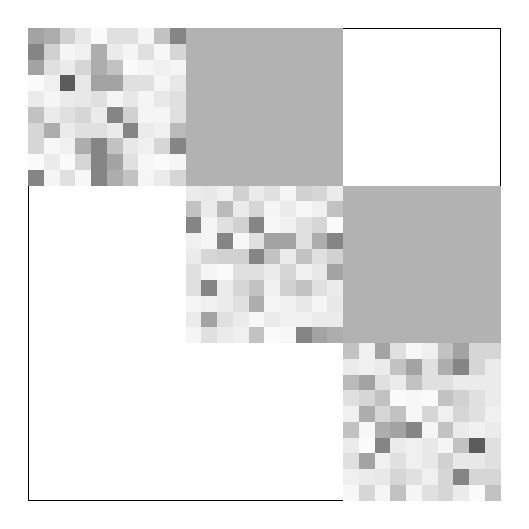
\begin{tikzpicture}[scale=0.2]
        \def\n{3}
        \def\k{10}

        \draw[black] (0,0) rectangle (\n*\k, \n*\k);

        \fill[black!30] (10, 20) rectangle ++ (\k, \k);
        \fill[black!30] (20, 10) rectangle ++ (\k, \k);
        
        \def\x{0}
        \def\y{20}
        \foreach \i in {1,...,\k} {
            \foreach \j in {1,...,\k} {
                % Calculate a shade between 10 and 90 based on position
                \pgfmathsetmacro{\shade}{random(4)*random(4)*random(4)}
                \fill[black!\shade] (\i + \x - 1, \j + \y - 1) rectangle ++ (1, 1);
            }
        }
        
        \def\x{10}
        \def\y{10}
        \foreach \i in {1,...,\k} {
            \foreach \j in {1,...,\k} {
                % Calculate a shade between 10 and 90 based on position
                \pgfmathsetmacro{\shade}{random(4)*random(4)*random(4)}
                \fill[black!\shade] (\i + \x - 1, \j + \y - 1) rectangle ++ (1, 1);
            }
        }
        
        \def\x{20}
        \def\y{0}
        \foreach \i in {1,...,\k} {
            \foreach \j in {1,...,\k} {
                % Calculate a shade between 10 and 90 based on position
                \pgfmathsetmacro{\shade}{random(4)*random(4)*random(4)}
                \fill[black!\shade] (\i + \x - 1, \j + \y - 1) rectangle ++ (1, 1);
            }
        }
    \end{tikzpicture}
    \subcaption{$\mathbf{W}_{rec}$ of a ML-ESM}
    \label{fig:ML_ESM_recurrence_matrix}
    \end{subfigure}
    ~
    \begin{subfigure}[t]{0.45\textwidth}
    \centering
    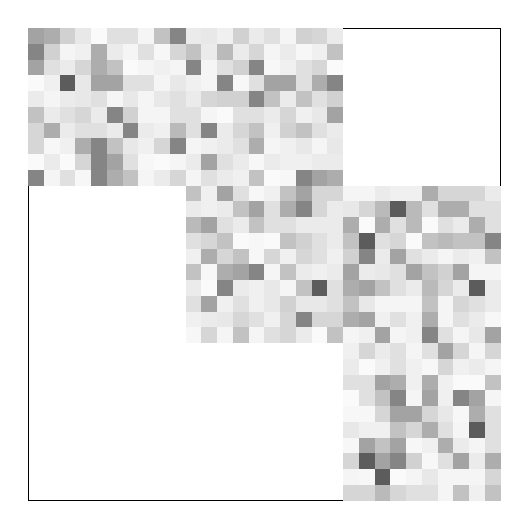
\begin{tikzpicture}[scale=0.2]
        \def\n{3}
        \def\k{10}

        \draw[black] (0,0) rectangle (\n*\k, \n*\k);
        
        \def\x{0}
        \def\y{20}
        \foreach \i in {1,...,\k} {
            \foreach \j in {1,...,\k} {
                % Calculate a shade between 10 and 90 based on position
                \pgfmathsetmacro{\shade}{random(4)*random(4)*random(4)}
                \fill[black!\shade] (\i + \x - 1, \j + \y - 1) rectangle ++ (1, 1);
            }
        }

        \def\x{10}
        \def\y{20}
        \foreach \i in {1,...,\k} {
            \foreach \j in {1,...,\k} {
                % Calculate a shade between 10 and 90 based on position
                \pgfmathsetmacro{\shade}{random(4)*random(4)*random(4)}
                \fill[black!\shade] (\i + \x - 1, \j + \y - 1) rectangle ++ (1, 1);
            }
        }
        
        \def\x{10}
        \def\y{10}
        \foreach \i in {1,...,\k} {
            \foreach \j in {1,...,\k} {
                % Calculate a shade between 10 and 90 based on position
                \pgfmathsetmacro{\shade}{random(4)*random(4)*random(4)}
                \fill[black!\shade] (\i + \x - 1, \j + \y - 1) rectangle ++ (1, 1);
            }
        }
        
        \def\x{20}
        \def\y{10}
        \foreach \i in {1,...,\k} {
            \foreach \j in {1,...,\k} {
                % Calculate a shade between 10 and 90 based on position
                \pgfmathsetmacro{\shade}{random(4)*random(4)*random(4)}
                \fill[black!\shade] (\i + \x - 1, \j + \y - 1) rectangle ++ (1, 1);
            }
        }
        
        \def\x{20}
        \def\y{0}
        \foreach \i in {1,...,\k} {
            \foreach \j in {1,...,\k} {
                % Calculate a shade between 10 and 90 based on position
                \pgfmathsetmacro{\shade}{random(4)*random(4)*random(4)}
                \fill[black!\shade] (\i + \x - 1, \j + \y - 1) rectangle ++ (1, 1);
            }
        }
    \end{tikzpicture}
    \subcaption{$\mathbf{W}_{rec}$ of a Deep-ESN}
    \label{fig:deep_ESN_recurrence_matrix}
    \end{subfigure}


    \caption{$\mathbf{W}_{rec}$ of ESN variants with sequential, feed-forward sub-reservoirs.}
    \label{fig:W_rec_sequential_ff}
\end{figure}

To compare against their Deep-ESN, Gallicchio and Micheli (2017) also introduced the Grouped-ESN in which the input signal is fed into several unconnected sub-reservoirs~\cite{gallicchio_and_micheli_2017}. The sub-reservoirs all contribute to the output, which is generated by a readout vector multiplied by the state of all of the sub-reservoirs. Its recurrence matrix is visualised in Figure \ref{fig:grouped_ESN_recurrence_matrix}. They created the Grouped-ESN to isolate the effect of the sequential stacking of sub-reservoirs in their Deep-ESN, and gauge the relative effect of splitting the reservoir into sub-reservoirs. Wcisło \& Czech (2021) built upon this idea by stacking multiple layers of parallel sub-reservoirs, forming what they called a Grouped Deep ESN (gdESN)~\cite{wcislo_2021}. Each sub-reservoir passes its states to its following sub-reservoir in the next layer. Where the regular ESN (with no bias vector) would update its state like so:
\[
    \mathbf{s}(t + 1) = f_{act}(\mathbf{W}_{in}\mathbf{x}(t) + \mathbf{W}_{rec}\mathbf{s}(t)).
\]
Any sub-reservoir after the first sub-reservoir $\mathbf{s}_{i + 1}(t)$ in a gdESN would update its states using the previous layer's states $\mathbf{s}_i(t)$ rather than the input $\mathbf{x}(t)$:
\[
    \mathbf{s}^{(i + 1)}(t + 1) = f_{act}(\mathbf{W}^{(i)}_{in}\mathbf{s}^{(i)}(t) + \mathbf{W}^{(i)}_{rec}\mathbf{s}^{(i + 1)}(t)).
\]

The nonlinearity introduced by the $f_{act}$ means the structure of gdESN can't be represented simply by restricting the recurrence weight matrix $\mathbf{W}_{rec}$, but rather as an ensemble of restricted ESNs. Another conception of the multi-reservoir ESN is the `Multiple-Reservoir Hierarchical ESN' (MH-ESN) proposed by Lun et al. (2023), which can be represented by restrictions to $\mathbf{W}_{rec}$~\cite{lun_2023}. The `layers' of the MH-ESN are not ordered sequentially, but instead represent groups of sub-reservoirs with similar parameter settings (number of nodes and sparsity). Each sub-reservoir in the MH-ESN has a single `principal' neuron, representing the average states of the neurons in that sub-reservoir. A visualisation of its recurrence matrix can be found in Figure \ref{fig:MH_ESN_recurrence_matrix}. MH-ESN differs to the Grouped-ESN because it sparsely connects the sub-reservoirs within each layer only using these principal neurons, where all other neurons are unconnected.

\begin{figure}
    \centering
    \begin{subfigure}[t]{0.45\textwidth}
    \centering
    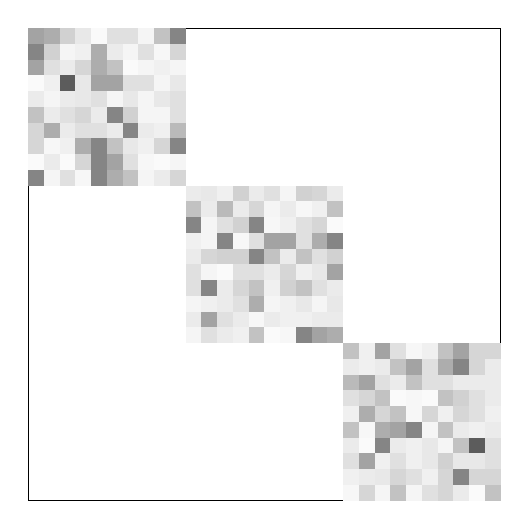
\begin{tikzpicture}[scale=0.2]
        \def\n{3}
        \def\k{10}

        \draw[black] (0,0) rectangle (\n*\k, \n*\k);
        
        \def\x{0}
        \def\y{20}
        \foreach \i in {1,...,\k} {
            \foreach \j in {1,...,\k} {
                % Calculate a shade between 10 and 90 based on position
                \pgfmathsetmacro{\shade}{random(4)*random(4)*random(4)}
                \fill[black!\shade] (\i + \x - 1, \j + \y - 1) rectangle ++ (1, 1);
            }
        }
        
        \def\x{10}
        \def\y{10}
        \foreach \i in {1,...,\k} {
            \foreach \j in {1,...,\k} {
                % Calculate a shade between 10 and 90 based on position
                \pgfmathsetmacro{\shade}{random(4)*random(4)*random(4)}
                \fill[black!\shade] (\i + \x - 1, \j + \y - 1) rectangle ++ (1, 1);
            }
        }
        
        \def\x{20}
        \def\y{0}
        \foreach \i in {1,...,\k} {
            \foreach \j in {1,...,\k} {
                % Calculate a shade between 10 and 90 based on position
                \pgfmathsetmacro{\shade}{random(4)*random(4)*random(4)}
                \fill[black!\shade] (\i + \x - 1, \j + \y - 1) rectangle ++ (1, 1);
            }
        }
    \end{tikzpicture}
    \subcaption{$\mathbf{W}_{rec}$ of a Grouped-ESN. The sub-reservoirs are not connected to one another, but internally are sparsely connected.}
    \label{fig:grouped_ESN_recurrence_matrix}
    \end{subfigure}
    ~
    \begin{subfigure}[t]{0.45\textwidth}
    \centering
    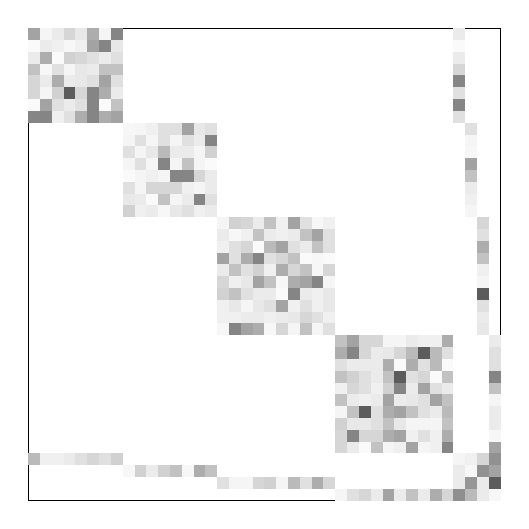
\begin{tikzpicture}[scale=0.15]
        \def\n{4}
        \def\k{10}

        \draw[black] (0,-10) rectangle (40, 30);

        \def\k{8}
        
        \def\x{0}
        \def\y{22}
        \foreach \i in {1,...,\k} {
            \foreach \j in {1,...,\k} {
                % Calculate a shade between 10 and 90 based on position
                \pgfmathsetmacro{\shade}{random(4)*random(4)*random(4)}
                \fill[black!\shade] (\i + \x - 1, \j + \y - 1) rectangle ++ (1, 1);
            }
        }
        
        \def\x{8}
        \def\y{14}
        \foreach \i in {1,...,\k} {
            \foreach \j in {1,...,\k} {
                % Calculate a shade between 10 and 90 based on position
                \pgfmathsetmacro{\shade}{random(4)*random(4)*random(4)}
                \fill[black!\shade] (\i + \x - 1, \j + \y - 1) rectangle ++ (1, 1);
            }
        }

        \def\x{0}
        \def\y{-6}
        \foreach \i in {1,...,\k} {
            % Calculate a shade between 10 and 90 based on position
            \pgfmathsetmacro{\shade}{random(4)*random(4)*random(4)}
            \fill[black!\shade] (\i + \x - 1, \y - 1) rectangle ++ (1, 1);
        }
        
        \def\x{\k}
        \def\y{-7}
        \foreach \i in {1,...,\k} {
            % Calculate a shade between 10 and 90 based on position
            \pgfmathsetmacro{\shade}{random(4)*random(4)*random(4)}
            \fill[black!\shade] (\i + \x - 1, \y - 1) rectangle ++ (1, 1);
        }
        
        \def\x{37}
        \def\y{22}
        \foreach \i in {1,...,\k} {
            % Calculate a shade between 10 and 90 based on position
            \pgfmathsetmacro{\shade}{random(4)*random(4)*random(4)}
            \fill[black!\shade] (\x - 1, \i + \y - 1) rectangle ++ (1, 1);
        }
        
        \def\x{38}
        \def\y{14}
        \foreach \i in {1,...,\k} {
            % Calculate a shade between 10 and 90 based on position
            \pgfmathsetmacro{\shade}{random(4)*random(4)*random(4)}
            \fill[black!\shade] (\x - 1, \i + \y - 1) rectangle ++ (1, 1);
        }

        \def\k{10}
        
        \def\x{16}
        \def\y{4}
        \foreach \i in {1,...,\k} {
            \foreach \j in {1,...,\k} {
                % Calculate a shade between 10 and 90 based on position
                \pgfmathsetmacro{\shade}{random(4)*random(4)*random(4)}
                \fill[black!\shade] (\i + \x - 1, \j + \y - 1) rectangle ++ (1, 1);
            }
        }
        
        \def\x{26}
        \def\y{-6}
        \foreach \i in {1,...,\k} {
            \foreach \j in {1,...,\k} {
                % Calculate a shade between 10 and 90 based on position
                \pgfmathsetmacro{\shade}{random(4)*random(4)*random(4)}
                \fill[black!\shade] (\i + \x - 1, \j + \y - 1) rectangle ++ (1, 1);
            }
        }
        
        \def\x{16}
        \def\y{-8}
        \foreach \i in {1,...,\k} {
            % Calculate a shade between 10 and 90 based on position
            \pgfmathsetmacro{\shade}{random(4)*random(4)*random(4)}
            \fill[black!\shade] (\i + \x - 1, \y - 1) rectangle ++ (1, 1);
        }
        
        \def\x{26}
        \def\y{-9}
        \foreach \i in {1,...,\k} {
            % Calculate a shade between 10 and 90 based on position
            \pgfmathsetmacro{\shade}{random(4)*random(4)*random(4)}
            \fill[black!\shade] (\i + \x - 1, \y - 1) rectangle ++ (1, 1);
        }
        
        \def\x{39}
        \def\y{4}
        \foreach \i in {1,...,\k} {
            % Calculate a shade between 10 and 90 based on position
            \pgfmathsetmacro{\shade}{random(4)*random(4)*random(4)}
            \fill[black!\shade] (\x - 1, \i + \y - 1) rectangle ++ (1, 1);
        }
        
        \def\x{40}
        \def\y{-6}
        \foreach \i in {1,...,\k} {
            % Calculate a shade between 10 and 90 based on position
            \pgfmathsetmacro{\shade}{random(4)*random(4)*random(4)}
            \fill[black!\shade] (\x - 1, \i + \y - 1) rectangle ++ (1, 1);
        }
        
        \def\x{36}
        \def\y{-10}
        \foreach \i in {1,...,\n} {
            \foreach \j in {1,...,\n} {
                % Calculate a shade between 10 and 90 based on position
                \ifnum\i=\j
                    \pgfmathsetmacro{\shade}{40 + random(4)*random(4)}
                \else
                    \pgfmathsetmacro{\shade}{random(4)*random(4)*random(4)}
                \fi
                \fill[black!\shade] (\i + \x - 1, \j + \y - 1) rectangle ++ (1, 1);
            }
        }
    \end{tikzpicture}
    \subcaption{$\mathbf{W}_{rec}$ of the MH-ESN. The principal node weights are in the bottom right. The sub-reservoirs are only connected to one another by their principal nodes.}
    \label{fig:MH_ESN_recurrence_matrix}
    \end{subfigure}


    \caption{$\mathbf{W}_{rec}$ of ESN variants with parallel sub-reservoirs.}
    \label{fig:W_rec_parallel}
\end{figure}

Throughout much of this literature, the authors stipulate that the advantage of multiple sub-reservoirs is to have a broad range of dynamics for the same input sequence, allowing the ESN to represent a broader and richer set of temporal features. In some cases, this is achieved by the \textbf{structure of the network}, as in the case of Jaeger's DFD, in which the input cascades through the different modules over time. This is similarly the case for the Deep-ESN, where each sub-reservoir passed the input signal along to the next sub-reservoir over time. The advantage afforded by a broad range of dynamics is achieved more explicitly by Babinec and Posp\'{\i}chal's modular ESN and for the Grouped-ESN, in which each sub-reservoir is \textbf{instantiated with different parameters} (for example, the spectral radius) to create differing properties such as memory capacity. Other modular ESNs use sequence resampling of the input signal (skipping, overlapping or segmenting) to supply each sub-reservoir with \textbf{different variations of the input time series}~\cite{li_tanaka_2021}. The different reservoirs are able to respond at multiple timescales for fast or slow dynamics and thus represent phenomena that requires more or less memory.




% - Other examples:
    % - Dual
    %     - Triefenbach et al. (2013)
    %         - Two 'sub-reservoirs', one receiving input in chronological order and one in reverse chronological
    %     - Ma et al. 2017b: Dual-Reservoir Network (DRN)
    %         - Two 'sub-reservoirs' are connected with an unsupervised encoder
    %         - The weights of the encoder are chosen using Principal Component Analysis
    % - aESN - Iinuma et al. (2022)
    % - reBASIC - Kawai et al. 2023a,b

\subsection{Context sensitive input routing}

By changing the structure of the recurrence matrix $\mathbf{W}_{rec}$, Dale (2018) introduced a `Reservoir of Reservoirs' architecture, comprising multiple sparsely connected sub-reservoirs linked by extremely sparse ($\approx$1\%) interconnections~\cite{dale_2018}. They evaluated two routing schemes: directing the input exclusively to a single sub-reservoir versus `broadcasting' it to all sub-reservoirs. On the NARMA benchmark, neither input routing scheme improved upon the traditional ESN, but the author showed that these architectures had a better transfer performance when retrained on unseen tasks (Santa Fe laser, noisy Hénon map). These ideas show the potential of input routing policies to shape reservoir performance and motivate the exploration of more flexible, context-sensitive input routing architectures.

It is possible to route the input signal to different sub-reservoirs depending on contextual information. Argentieri et al. (2022) proposed the Input Routed Echo State Network (IR-ESNs) to improve the prediction of ESNs on multi-dimensional signals~\cite{argentieri_2022}. When the input signal $\mathbf{x}(t)$ is a vector rather than a scalar, traditional ESNs process all input dimensions within a single reservoir. Argentieri et al. argued that this can lead to the mixing of distinct input features and potentially obscure the individual characteristics of each input dimension.

To overcome this limitation, the authors proposed an architecture that routes different dimensions of the input signal to dedicated sub-reservoirs within a multi-reservoir model. Each sub-reservoir receives only a specific component of the input and so develops dynamics reflecting those components separately. Additionally, the sub-reservoirs are interconnected, enabling the modelling of interactions between different input dimensions as required by the task. The authors evaluated their IR-ESNs on both synthetic and real-world time series classification problems. They demonstrated that IR-ESNs outperform standard ESNs in predicting multi-dimensional signals, showing that the proposed routing mechanism leverages the distinct characteristics of each input dimension.



\section{Readout switching}

While there are many examples of ESNs with a partitioning of the reservoir, researchers have also explored ESNs where partitioning focuses on the readout function. For example, Ma \& Chen (2013) conceived of a `Modular State Space ESN (MSSESN)' by dividing the reservoir in the high-dimensional coordinate space of its states (state space), rather than dividing the internal weight matrix of the reservoir~\cite{ma_chen_2013}. They achieved this by fitting a piecewise readout function, with a separate linear readout for each module. They partition the state space by partitioning predictions derived from the reservoir, arguing that the Euclidean norm of any two states is likely proportional to the Euclidean norm of any two predictions. The state space is divided by first fitting an ordinary linear readout on the reservoir, $\mathbf{C}_{out}$, and then performing an equal partitioning of the predictions generated from this linear readout such that $h_i \leqslant \mathbf{C}_{out}\mathbf{s}(t) < h_{i+1}$ where $h_i$ and $h_{i+1}$ are the bounds of each partition. The partitioning of the predictions gives a partitioning of their state space values, since any unseen reservoir state can be allocated a partition based on its evaluation of $\mathbf{C}_{out}\mathbf{s}(t)$. Then a new readout $\mathbf{C}_{out}^{(k)}$ can be fitted for each partition $k$, providing a specific readout for each partition of state space. Thus, the piecewise linear readout function is driven by the states of the reservoir itself and was shown to improve prediction performance on non-stationary time series.

Laan \& Vicente (2015) also proposed an ESN with multiple linear readout modules, where a module is chosen depending on the states of the reservoir~\cite{laan_vicente_2015}.
Each module has two vectors: a readout vector and a weighting vector.
The readout vector is fitted via regression while the weighting vector is randomly instantiated.
Each module makes its own prediction by taking the scalar product of the readout vector and the states of the network - as a traditional ESN would.
Each module also makes its weighting by taking the scalar product of its weighting vector and the states of the network.
The predictions from each module are then combined in a softmaxed weighted sum using their weights. 
Thus the relative weights of each module change according to how the states change over time, emphasising some modules at some times and others at other times.

\vspace{1em}

The architectures reviewed in this chapter illustrate the diverse ways in which modularity can be incorporated into ESNs. Components such as input routing, restricted reservoirs and readout switching offer options for creating novel model architectures. These components not only increase the variety of models we can apply to any prediction task, but also allow us to incorporate specific features of data into the architecture of ESNs. In the following chapters, we treat each of these architectural elements as potential building blocks for developing ESNs that leverage ordinal partitions as a key feature, with the aim of enhancing predictive performance.


